\startfirstchapter{Introduction}
\label{chapter:introduction}
This work contributes empirical results to support parameterization of grab and
release actions.
The high level goal of this research is to improve quality of human computer interaction using hands.
It is not difficult to observe in daily life that interaction with computers using hands is far more limited compared to how we manipulate and interact with the physical world around us.
Many people are capable of -- and enjoy -- performing complex asynchronous bimanual tasks such as playing the guitar, throwing clay pots, and carving wooden sculptures.
I believe lack of accurate parameterization of hand actions is one of the primary obstacles against incorporating support for such rich hand interactions within software applications.

Most contemporary multi-touch devices only receive and use contact information with the surface.  
This approach limits sensing bandwidth, making it very difficult or impossible to recognize what type of motion a user is performing with their hand on near the surface.  
Furthermore, due to the lack of any hand tracking in most contemporary systems, it is not possible to assign modes or states to the hands.  
These limitations hinder the design of bimanual as well as co-located collaborative interfaces.
%Focus on the empirically validated techniques to parameterize and implement multitouch and near touch gestures; this is what we should be introducing; your hardware & s/w is a cool apparatus to accomplish your parameterization research contributions

\begin{figure}[t!]
 \centering
 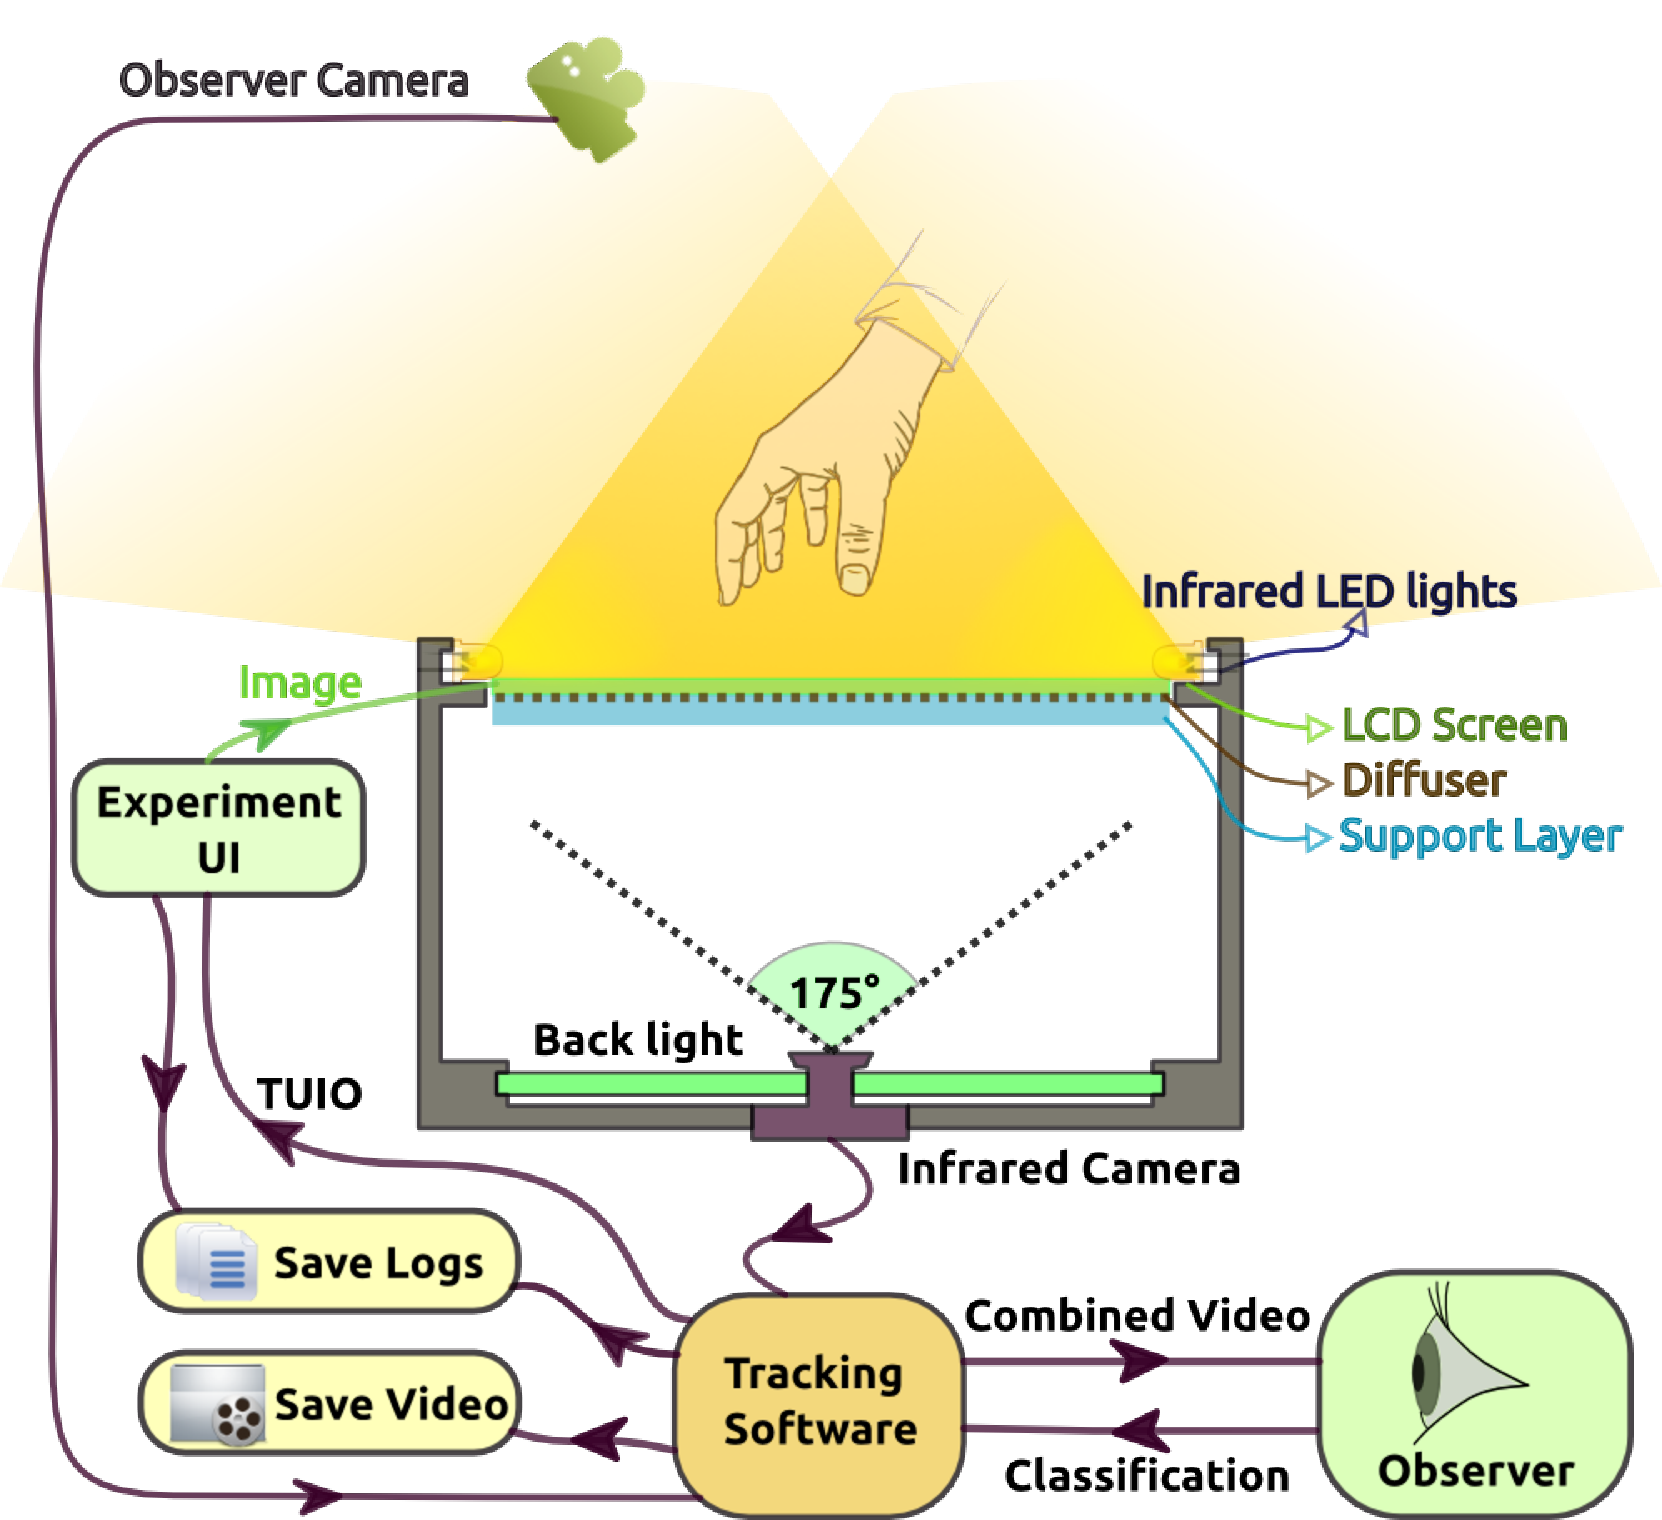
\includegraphics[type=pdf,ext=.pdf,read=.pdf,width=5in]{./img/neartouch_prototype.png}
 \caption[Interplay between the hardware and software components of my system to process near touch interactions.]{
Interplay between the hardware and software components of my system to process near touch interactions.
Tracking software receives frames from both an infrared camera and an observer camera.
Only frames from the infrared camera are processed by computer vision algorithms.
The frames from the two cameras are combined into one video stream that are superimposed with annotations.
This video stream was shown to the wizard operating the Wizard of Oz system, and was stored in real time for post study analyses.
The actions recognized by the wizard are sent to the tracking software by pressing shortcut keys, which in turn each trigger an event to send a TUIO message to the experiment UI in front of the participant.
Both the tracking software and the experiment UI save a record in their own CSV log file containing all the data relevant to the current task.
In addition to these two log files, tracking software records an OpenCV YML file containing a feature matrix with all available information from the temporal window prior to performing the task.
This data can be used for training classification algorithms in future research.
% Can we make this data available for download somewhere?  Or, do we wish to save it, perform our own training classification algorithm research, and then make the data public?
}
 \label{fig:neartouch_prototype}
\end{figure}

\section{Guiding Research Questions}
Existing research projects that explore near touch surface interactions mostly focus on developing novel hardware solutions or the design of new interactions.
In addition to building upon related systems research, the current work presents empirically validated techniques that can be applied to future systems and interaction techniques.  
This work is guided by the following research questions.  
\begin{enumerate}
\item What is an appropriate, accurate model for detecting the center of a user's  action? 
In other words, where should a hand action (for example grab) be applied to so it is closest to where a user expects?
\item What data from typical tracking software is needed to accurately model the actions performed by users and what size of temporal window would be appropriate for collecting these data?
\end{enumerate}

\begin{figure}[t!]
 \centering
 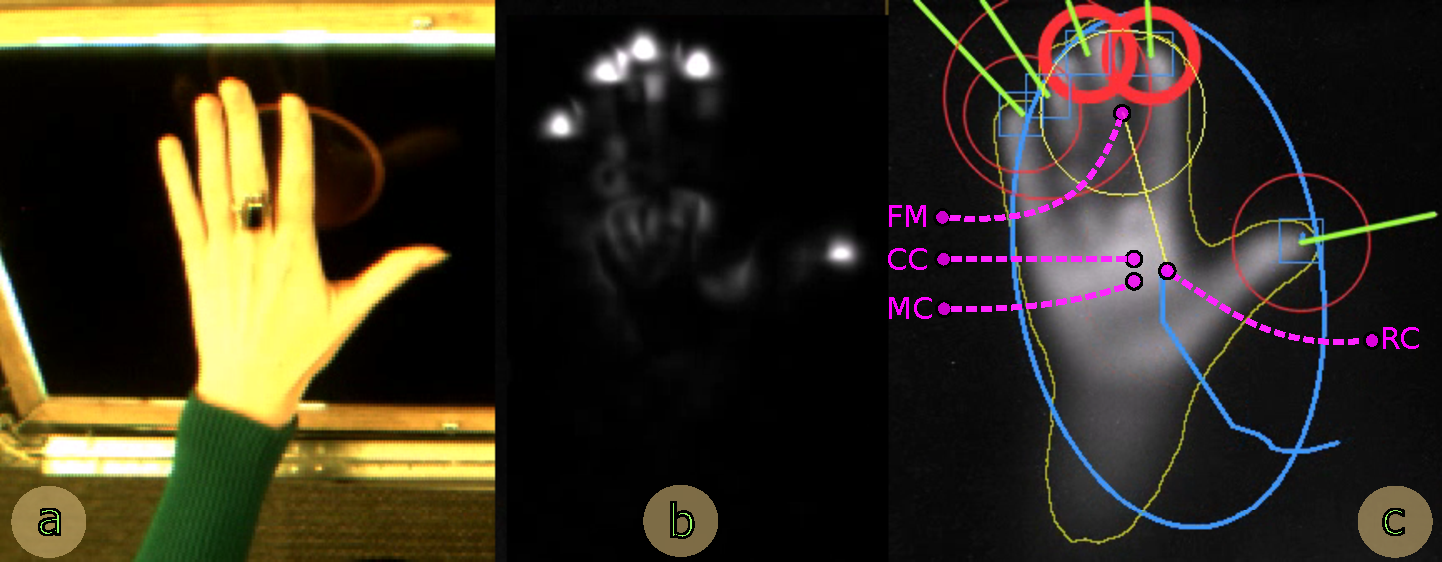
\includegraphics[width=6in]{./img/teaser/teaser.pdf}
 % teaser.pdf: 692x270 pixel, 72dpi, 24.41x9.52 cm, bb=0 0 692 270
 \caption[Three views of my near touch processing for a user's hand]{ Three views of my near touch processing for a user's hand:  
\textbf{a)} a snapshot of a participant's hand after releasing an object on a target,
\textbf{b)} the intermediate sharpness image used to approximate depth of prominent hand features such as finger tips, and
\textbf{c)} the hand image as viewed through an infrared camera mounted behind the LCD display; 
colored annotations illustrate processing results by my system; the thin yellow line represents to the outline of the hand; 
the thin red circles represent fingertips near the surface but not touching; the bold red circles represent finger touches; 
the green lines represent finger orientation with respect to rectangle center; the thin blue line represents the bounding oval used to estimate the hand's center of mass; 
the magenta labels represent the four independent parameters used in my study -- (i) minimum enclosing circle center (CC), (ii) minimum enclosing rectangle center (RC), (iii) feature mean location (FM) and (iv) center of mass (MC).
}
 \label{fig:teaser}
\end{figure}

\section{Near Touch Apparatus Summary}
I introduce a prototype multi-touch and near touch tracking system (see Figure \ref{fig:neartouch_prototype}).  
I chose a rear mounted camera setup for my hardware prototype because I believe recent advances in display technology, including advances in manufacturing OLED (Organic Light-Emitting Diode) displays, will lead to a new generation of display technologies that are capable of capturing an image of what is directly in front of the display.  
For example, Hirsch et al.'s \cite{Hirsch:2009:BIDI} BiDi screen is a thin depth sensing prototype that demonstrates feasibility of manufacturing for future systems using a grid of pinhole cameras embedded inside a flat display.  
My choice of hardware deals with relatively similar types of signals as Hirsch et al. and can therefore contribute to future near touch sensing technologies in terms of hardware implementation, image processing, and interaction design.

\section{Empirical Findings Summary}
The main focus of this study is to find the most accurate model that would identify the center of grab and release actions performed by a user.  
Before we can create a model for the center of the hand, we need to identify what factors most influence a user's interactions.  
To find this information, I conducted a user study where participants performed grab and release actions on an experiment interface using my near touch apparatus. Figure \ref{fig:teaser} demonstrates main features of this apparatus.

Using dependent variables from the user study and based on my initial observation of users, I formulate four primary models to predict the center of users' actions.
The dependent variables are parameters extracted from images of the hand in real time from a temporal window prior to performing the action. 
The performance of the proposed models were very similar, suggesting a high-level robustness in my approach.  
Another important finding of my study is an approach for distinguishing left and right hands when an action of grab or release has been registered.  
These center of action and hand distinction findings are detailed in the Results section.

%\pagebreak
